\documentclass{beamer}
\usepackage{graphicx,proof}
\usetheme{Boadilla}
\usecolortheme{beetle}

\newcommand{\G}{\Gamma}
\newcommand{\D}{\Delta}
\newcommand{\entails}{\vdash}
\newcommand{\rulename}[1]{\text{\textsc{(#1)}}}

\title{Group Therapy for the Type-Curious}
\subtitle{Theory \& Practice}
\author{Bruce C. Miller}
\institute{bm3719@gmail.com}
\date{November 14, 2018}

\begin{document}

\begin{frame}
  \titlepage
\end{frame}

\begin{frame}
  \frametitle{Our Noble Journey}
  \centerline{
\includegraphics[scale=0.4]{img/transformation.png}}
\end{frame}

\begin{frame}
  \frametitle{Overview}
  \begin{description}
  \item[Type Theory] Introduction and fundamentals
  \item[Type Systems] Type theory applied to programming languages
  \item[Static vs. Dynamic] And other dichotomies
  \item[Types vs. Clojure] Begun, the Type Wars have
  \end{description}
\end{frame}

\begin{frame}
  \frametitle{History of Type Theory}
  Some History:
  \begin{description}
  \item[1902] Types are first proposed by Bertrand Russell as a solution to
    Russell's Paradox in Cantor's na{\"i}ve set theory.
  \item[1940] Types are first applied to programming language theory, combined
    with Alonzo Church's $\lambda$-calculus.
  \item[1972] System F created.  Later to influence ML, Caml, Haskell.
  \item[1972] Per Martin-L{\"o}f's intuitionistic type theory introduced.
    Creates what's now known as dependent type theory, as used in Agda, Idris,
    Coq, Lean.
  \item[2009] What is now known as homotopy type theory introduced in a paper
    by Voevodsky.
  \end{description}
\end{frame}

\begin{frame}
  \frametitle{Type Judgments}
  \fbox{An introduction to type theory, just as relates to type systems.}\\
  \vspace{20pt}
  Judgments describe type systems.\\
  \[ \G \entails \Im \]\\
  $\Im$ is an assertion. $\Gamma$ here is the static typing environment, and
  could be the empty set $\emptyset$, or a list of variables and their types.\\
  \[ \G \entails \textit{M} : \textit{A} \]\\
  \textit{M} has type \textit{A} in $\Gamma$.\\
  \[ \emptyset \entails \textit{true} : \textit{Bool} \]
  \[ \G \entails \Diamond \]
\end{frame}

\begin{frame}
  \frametitle{Type Rules and Derivations}
  \vspace{20pt}
  Judgments compose type rules, which compute type derivations.\\
  \vspace{10pt}
  General form:
  \[ \infer[(Rule\:name)(annotations)]{\Gamma \entails \Im}{\Gamma_1 \entails \Im_1
      \ldots \Gamma_n \entails \Im_n} \]
  Some examples:
  \vspace{2pt}
  \[ \infer[(Env\:\emptyset)]{\emptyset \entails \Diamond}{} \]
  \vspace{2pt}
  \[ \infer[(Val\:\textit{n})(\textit{n} = 0,1,\ldots)]{\G \entails n :
      \textit{Nat}}{\G \entails \Diamond} \]
  \vspace{2pt}
  \[ \infer[(Val\:+)]{\G \entails \textit{M} + \textit{N} : \textit{Nat}}{\G
      \entails \textit{M} : \textit{Nat}, \G \entails \textit{N} : \textit{Nat}} \]
\end{frame}

\begin{frame}
  \frametitle{Type Systems}
  From Pierce \cite{TAPL}:\\
  \textit{A type system is a tractable syntactic method for proving the absence
    of certain program behaviors by classifying phrases according to the kinds
    of values they compute.}\\
  \vspace{20pt}
  Some notes:\\
  \begin{itemize}
    \item Languages without type systems are untyped.
    \item Type systems are parts of programming languages or can be implemented
      on their own.
    \item The line between the type system and general language implementation
      can be fuzzy, e.g. duck typing, type coercion.
    \item Type safety is the degree to with a language enforces the prevention
      of type errors.
  \end{itemize}
\end{frame}

\begin{frame}
  \frametitle{Type Dichotomies}
  \centerline{
    \begin{tabular}{|p{3cm}||p{3cm}|}
      \hline
      typed&untyped\\
      \hline
      static&dynamic\\
      \hline
      explicit&implicit\\
      manifest&inferred\\
      \hline
      structural&nominal\\
      \hline
      sound&unsound\\
      \hline
      intrinsic&extrinsic\\
      \hline
    \end{tabular}}
  \vspace{20pt}
  There are some conversational dichotomies that don't really have firm
  definitions:\\
  \centerline{
    \begin{tabular}{|p{3cm}||p{3cm}|}
      \hline
      weak&strong\\
      \hline
      loose&tight?\\
      \hline
    \end{tabular}}
\end{frame}

\begin{frame}
  \frametitle{The Static Typing Position}
  Aggregated from Haskell user opinions:
  \begin{itemize}
  \item \textbf{Reduction in bugs} Detection at compile time.  Closed vs. open
    programs.
  \item \textbf{Communicating intent} Type signatures, type declarations, etc.
  \item \textbf{Encoding program logic} Making bugs into type errors, refactoring.
  \item \textbf{Easier for n00bs} Naming nouns, nouns describe what they are/do.
  \item \textbf{Esoterica} Type-level programming, C-H, CT, etc.
  \end{itemize}
\end{frame}

\begin{frame}
  \frametitle{The Dynamic Typing Position}
  Aggregated from Clojure user opinions:
  \begin{itemize}
  \item \textbf{Real world data} In real life, data is sparse and/or unstructured.
  \item \textbf{Syntactic overhead} Code density, reduced logic distribution,
    small-scale development, REPLs.
  \item \textbf{Ease of Maintenance} Adding to and refactoring code.
  \item \textbf{Lazy-loading needed parts} spec, core.typed, core.logic
  \item \textbf{Type errors vs. real life} Clojure ranks as one of the lowest
    bug-prone languages.
  \end{itemize}
\end{frame}

\begin{frame}
  \frametitle{Resources}
  \begin{thebibliography}{9}
  \bibitem{talk} \emph{Group Therapy for the Type-Curious},
    \url{https://github.com/bm3719/types-talk}.
  \bibitem{TTFP} R. Nedepelt, H. Geuvers, \emph{Type Theory and Formal Proof: An
      Introduction}, 1st Edition, Cambridge Univ. Press, Cambridge, MA, 2014.
  \bibitem{TAPL} B. Pierce, \emph{Types and Programming Languages}, MIT
    Press, Cambridge, MA, 2002.
  \bibitem{PandT} J. Girard, \emph{Proofs and Types}, Cambridge Tracts on
    Comp. Sci., Cambridge, MA, 1989.
  \bibitem{ATTAPL} B. Pierce, \emph{Advanced Topics in Types and Programming
      Languages}, MIT Press, Cambridge, MA, 2004.
  \end{thebibliography}
\end{frame}

\begin{frame}
  \frametitle{Languages compared}
  Languages sorted by bug density (100+ star repos):\\
  \vspace{10pt}
  \centerline{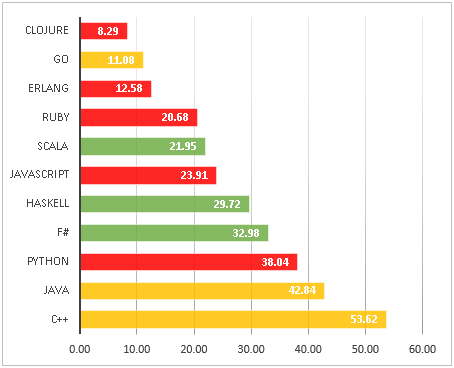
\includegraphics[scale=0.4]{img/bug_density.png}}
  \footnotesize{
  \begin{flushright}
    https://dev.to/danlebrero/the-broken-promise-of-static-typing
  \end{flushright}
  }
\end{frame}

\begin{frame}
  \frametitle{The Rosetta Stone}
  \footnotesize{
  \centerline{
    \begin{tabular}{|c||c||c||c||c|}
      \hline
      Category Theory&Physics&Topology&Logic&Computation\\
      \hline
      object X&Hilbert space X&manifold X&proposition X&data type X\\
      \hline
      morphism&operator&cobordism&proof&program\\
      $\textit{f}: \textit{X} \rightarrow \textit{Y}$&
      $\textit{f}: \textit{X} \rightarrow \textit{Y}$&
      $\textit{f}: \textit{X} \rightarrow \textit{Y}$&
      $\textit{f}: \textit{X} \rightarrow \textit{Y}$&
      $\textit{f}: \textit{X} \rightarrow \textit{Y}$\\
      \hline
      tensor product&Hilbert space&disjoint union&conjunction&product\\
      of objects:&of joint system:&of manifolds:&of propositions:&of data
                                                                   types:\\
      $\textit{X}\otimes\textit{Y}$&$\textit{X}\otimes\textit{Y}$&$\textit{X}\otimes\textit{Y}$&$\textit{X}\otimes\textit{Y}$&$\textit{X}\otimes\textit{Y}$\\
      \hline
    \end{tabular}}
  }
\end{frame}

\begin{frame}
  \frametitle{The Rosetta Stone: Homotopy Types}
  \footnotesize{
  \centerline{
    \begin{tabular}{|l l l l|}
      \hline
      Types&Logic&Sets&Homotopy\\
      \hline
      \textit{A}&proposition&set&space\\
      \textit{a}:\textit{A}&proof&element&point\\
      \textit{B}(\textit{x})&predicate&family of sets&fibration\\
      \textit{b}(\textit{x}):\textit{B}(\textit{x})&
      conditional proof&family of elements&section\\
      0,1&$\bot,\top$&$\emptyset,\{\emptyset\}$&$\emptyset,*$\\
      $A + B$&$A \vee B$&disjoint union&coproduct\\
      $A \times B$&$A \wedge B$&set of pairs&product space\\
      $A \rightarrow B$&$A \Rightarrow B$&set of functions&function space\\
      $\sum_{(\textit{x}:\textit{A})}\textit{B}(\textit{x})$&$\exists_{\textit{x}:\textit{A}}\textit{B}(\textit{x}$&disjoint sum&total space\\
      $\prod_{(\textit{x}:\textit{A})}\textit{B}(\textit{x})$&$\forall_{\textit{x}:\textit{A}}\textit{B}(\textit{x})$&product&space of sections\\
      $id_{\textit{A}}$&equality =&$\{ (x,x) | x \in A\}$&path space $\textit{A}^I$\\
      \hline
    \end{tabular}}
  }
\end{frame}

\end{document}
